\section{GPU Implementation} \label{gpu-implementation}
The temporal consistency that can be achieved using the described method is
usable for many applications, however as the optical flow is always needed for
temporal filtering it is calculated no matter which application is implemented.
Optical flow by itself can be used used for various applications like frame
interpolation, motion blur or motion magnification
\cite{journals/tog/LiuTFDA05}.

\paragraph{Disparity Estimation} \label{disparity-estimation}
Disparity estimation is about computing the correspondence between a pair of
stereoscopic images. The result $J_{xy}=d_{xy}$ can be used as depth map for
various tasks. Finding correspondences in stereoscopic images is very similar to
calculating optical flow from consecutive video frames:
\begin{align*}
  E_{data}(d) &= \sum_{(x,y)}\norm{I^r(x + d_{xy}, y) - I^l(x,y)}^2\\
  E_{smooth}(d) &= \sum_{(x,y)}\left( \norm{\nabla d_{xy}} \right)^2
\end{align*}
$J$ is sparsely initialized by feature matches between $I^r$ and $I^l$ and then
filtered as it was done for optical flow. \autoref{fig:disparity} shows an
example.
\begin{figure}[htb]
  \centering
  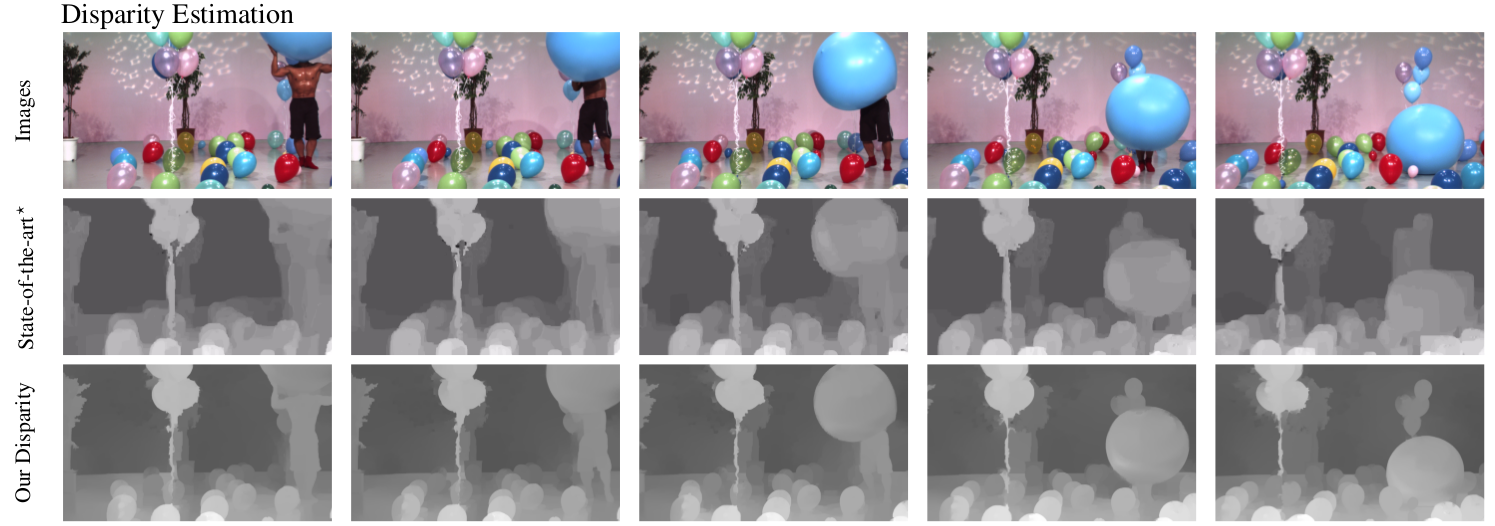
\includegraphics[width=0.5\textwidth]{images/disparity.png}
  \caption{The results of the disparity estimation is compared of a state of the
  art dataset provided by the MPEG group for testing. Again the results of the
proposed method is more stable in time. Less holes are randomly appearing and
disappearing compared to MPEG data set.}
  \label{fig:disparity}
\end{figure}

\paragraph{Colorization and Scribble Propagation} \label{colorization}
The approach can be used to propagate user input (pen strokes) through a given
video. The scribbles can have arbitrary meaning like color input for
colorization or ids for object labeling. The input scribbles $s_j$ from frame
$j$ are used to initialize $J_j = s_j$. Then the joint temporal smoothing is
applied to create intermediate frames. In average only every 20th frame needs
own scribble data.  \autoref{fig:scribble} shows an example for this
application.

\paragraph{Depth up-sampling} \label{up-sampling}
Depth sensor data from devices like Microsoft Kinects often suffer from bad
resolution, temporal noise and holes. The authors use their technique to filter
this data ($J$) using the image data from the Kinects camera for the domain
transform. As a result $J'$ is getting up-sampled, holes are getting filled and
noise is smoothed. \autoref{fig:depth-upsampling} shows a before-after
comparison.
\begin{figure}[htb]
  \centering
  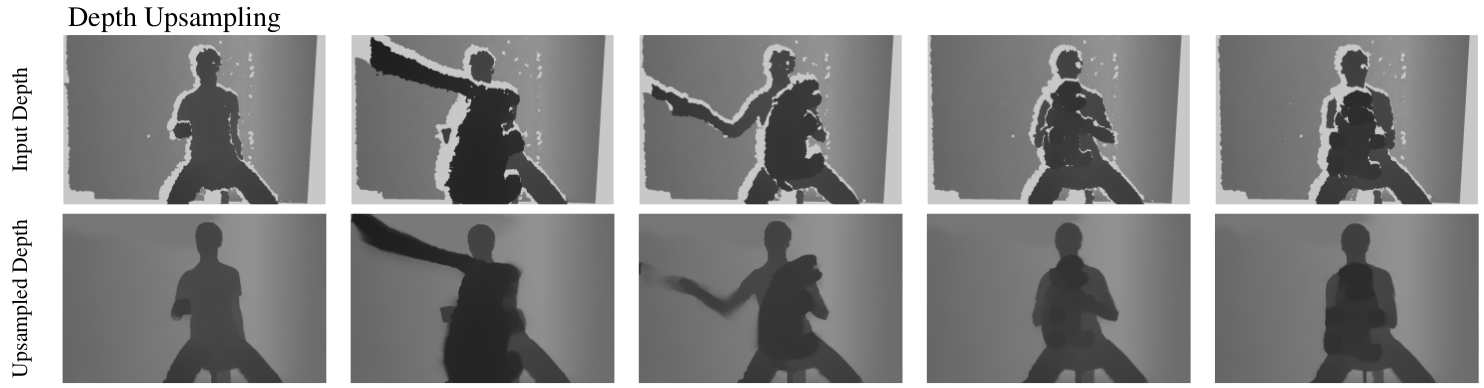
\includegraphics[width=0.5\textwidth]{images/depth.png}
  \caption{Low resolution and extremely noisy depth maps from a Microsoft Kinect
  is up-sampled and filled (white holes) using the same joint filtering
operation as it is used for the optical flow calculation. The image data from
the Kinect camera is used for the domain transform.}
  \label{fig:depth-upsampling}
\end{figure}

\paragraph{Saliency} \label{saliency}
Visual saliency maps are used in many graphics applications as they highlight
important regions in images. They can be used to change the aspect ratio of a
video without distorting important features (persons). In this case temporal
inconsistencies show up as wobbling. The authors used a per frame saliency
calculation $l$ as initialization for $J(x,y) = l(x,y)$ and applied the temporal
smoothness operation to gain consistent results. \autoref{fig:saliency} shows
the difference between the unfiltered and the filtered saliency.
\begin{figure}[htb]
  \centering
  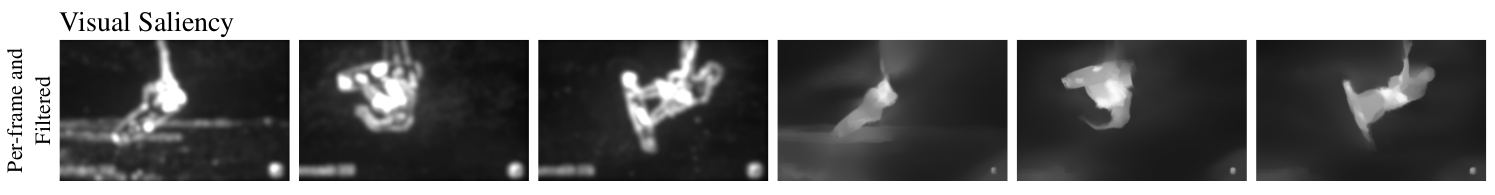
\includegraphics[width=0.5\textwidth]{images/saliency.png}
  \caption{First three images show the per frame saliency calculation, which are
  then temporally filtered to create the smooth results on the right.}
  \label{fig:saliency}
\end{figure}

